%Ne pas numéroter cette partie
\part*{Annexes}
%Rajouter la ligne "Annexes" dans le sommaire
\addcontentsline{toc}{part}{Annexes}



\begin{table}[ht]
\centering

\begin{longtable}{ |l|l|l| }
\hline
\multicolumn{2}{ |c| }{Acteurs du système} \\
\hline
Utilisateur  & Attributs \\ \hline

\multirow{11}{*}{Medecin}  
&  Id        \\        
&  Nom \\
& Prénom \\
& Organisme \\ 
& Spécialité \\
&  CIN \\
& Sexe \\
& Téléphone \\ 
& Email \\
& Adresse \\
& Mot de passe \\ 


  \hline
\multirow{11}{*}{Patient} 
  & Id  \\
  & Nom \\
  & Prénom \\
  & CIN \\ 
&   Sexe  \\
&   Téléphone \\
&   Email \\
&   Adresse \\
&   Date de naissance \\
&   Rendez-vous \\
&   Historique \\
&   Mot de passe \\  \hline

  
\multirow{2}{*}{Administrateur}  
  & Id \\
  & Mot de passe  \\  \hline
 
 
\multirow{11}{*}{Radiologue}  
&  Id     \\        
&  Nom \\
& Prénom \\
& Organisme \\ 
& Spécialité \\
& CIN \\
& Sexe \\
& Téléphone \\ 
& Email \\
& Adresse \\
& Mot de passe \\  \hline
 

\end{longtable}

\caption{Acteurs du système.}
\label{table:acteurstest}
\end{table}








\begin{table}[h!]
\centering
\begin{tabular}{lc}
\hline
\multicolumn{1}{|c|}{Utilisateurs}            & \multicolumn{1}{c|}{Attributs} \\ \hline
\multicolumn{1}{c}{\multirow{11}{*}{Médecin}} & Id                             \\
\multicolumn{1}{c}{}                          & Nom                            \\
\multicolumn{1}{c}{}                          & Prénom                         \\
\multicolumn{1}{c}{}                          & Organisme                      \\
\multicolumn{1}{c}{}                          & Spécialité                     \\
\multicolumn{1}{c}{}                          & CIN                            \\
\multicolumn{1}{c}{}                          & Sexe                           \\
\multicolumn{1}{c}{}                          & Téléphone                      \\
\multicolumn{1}{c}{}                          & Email                          \\
\multicolumn{1}{c}{}                          & Adresse                        \\
\multicolumn{1}{c}{}                          & Mot de passe                   \\
\multirow{12}{*}{Patient}                     & Id                             \\
                                              & Nom                            \\
                                              & Prénom                         \\
                                              & CIN                            \\
                                              & Sexe                           \\
                                              & Téléphone                      \\
                                              & Email                          \\
                                              & Adresse                        \\
                                              & Date de naissance              \\
                                              & Rendez-vous                    \\
                                              & Historique                     \\
                                              & Mot de passe                   \\
\multirow{2}{*}{Administrateur}               & ID                             \\
                                              & Mot de passe                   \\
\multirow{9}{*}{Radiologue}                   & ID                             \\
                                              & Nom                            \\
                                              & Prénom                         \\
                                              & CIN                            \\
                                              & Sexe                           \\
                                              & Téléphone                      \\
                                              & Email                          \\
                                              & Adresse                        \\
                                              & Mot de passe                  
\end{tabular}

\caption{Acteurs du système.}
\label{table:acteurs}

\end{table}




\subsection{Profile du patient}

\begin{figure}[!h]
\centering
\begin{center}
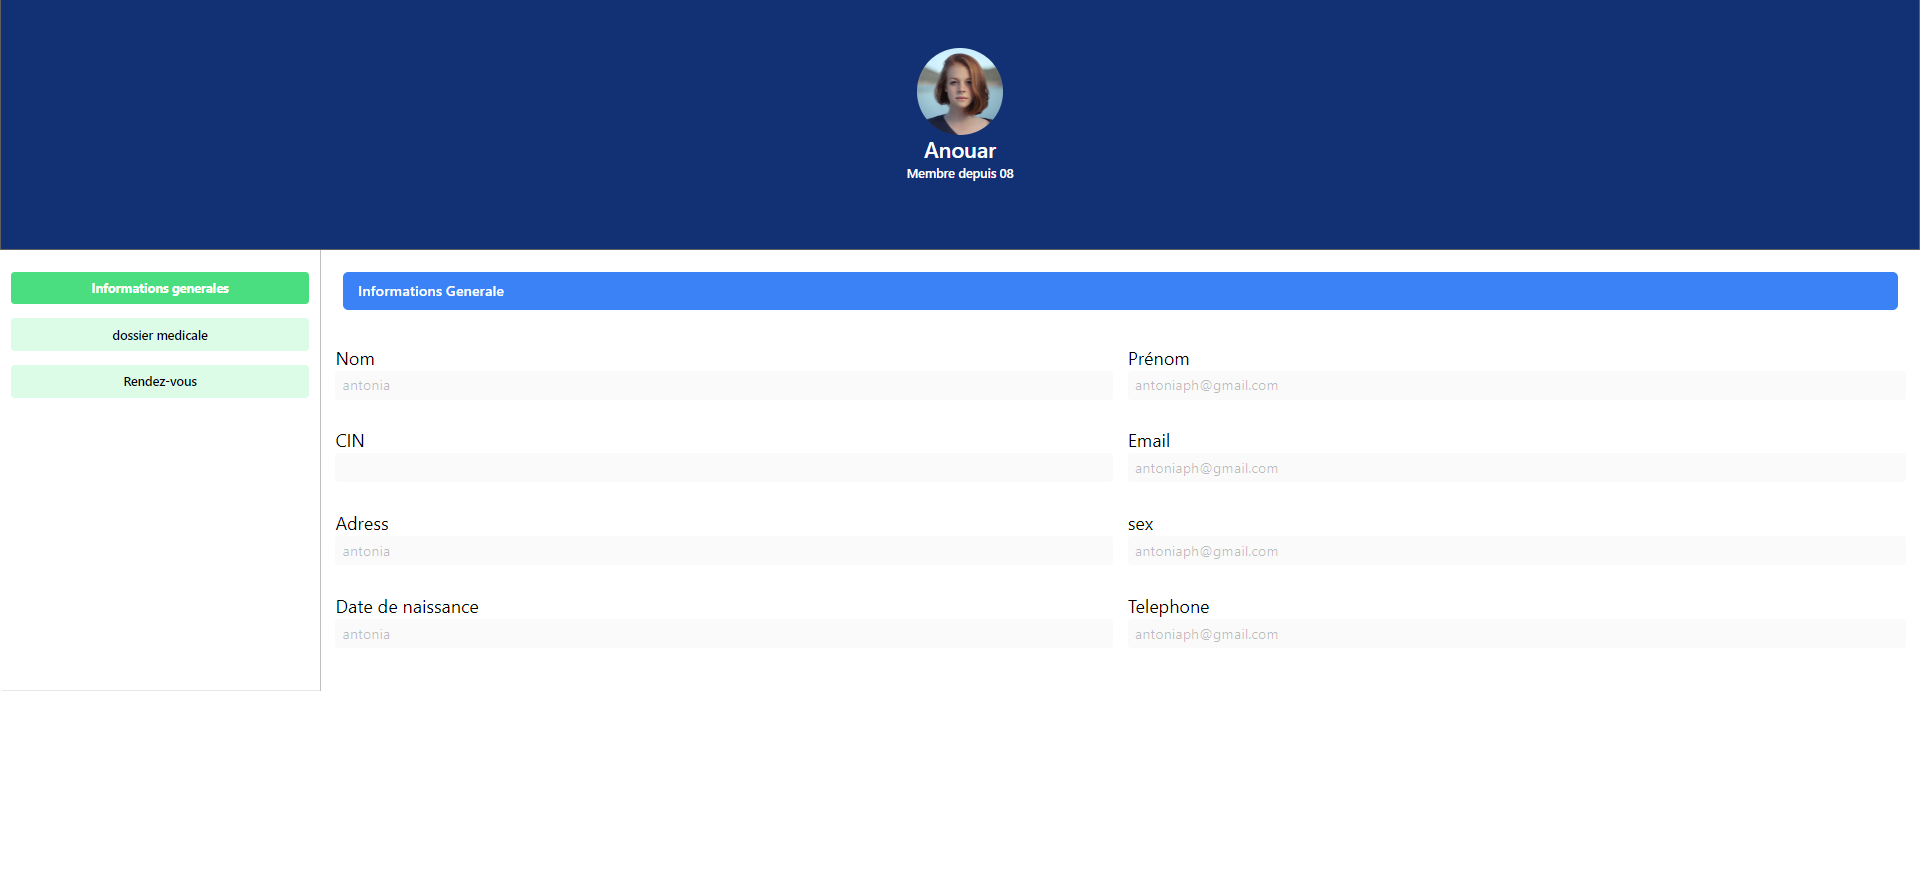
\includegraphics[height=10cm,width=18cm]{gen.png}
\end{center}
\caption{Profile du patient}
\end{figure}

\subsection{Dossier medical du patient}


\begin{figure}[!h]
\begin{center}
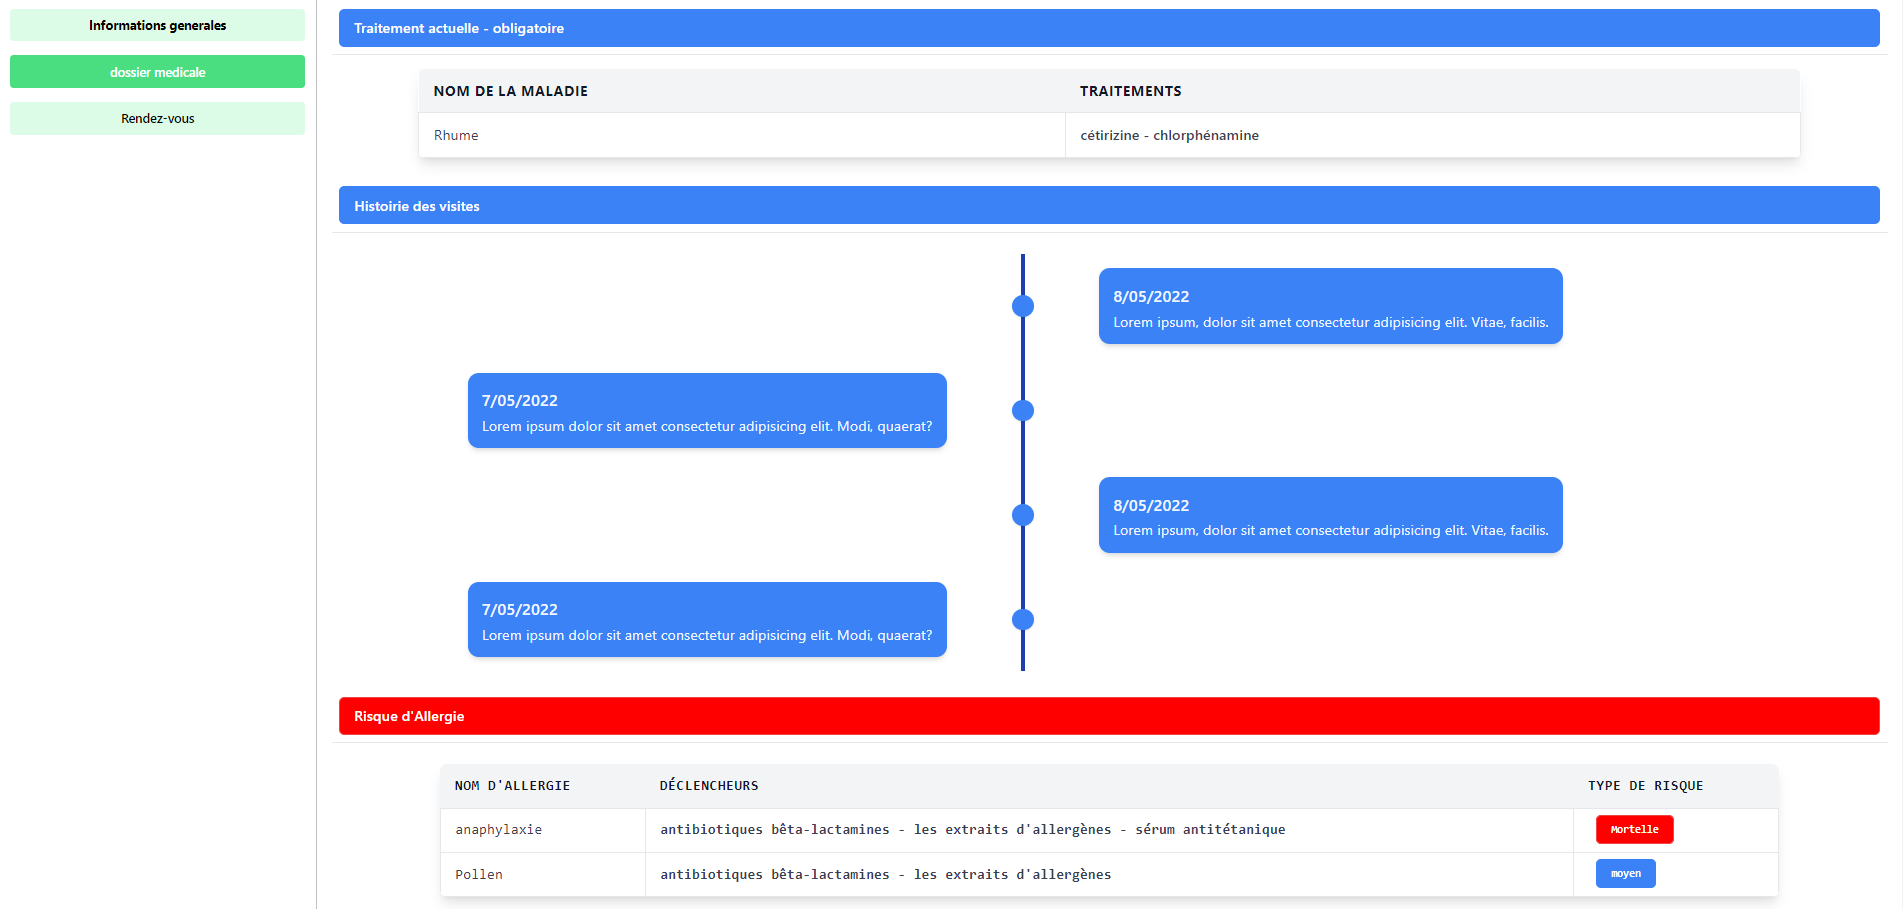
\includegraphics[height=8cm,width=18cm]{med.png}
\end{center}
\caption{Dossier medical du patient}
\end{figure}




\input{./annexe1.tex}

\input{./annexe2.tex}